\documentclass[aspectratio=169,dvipsnames]{beamer}
\usetheme{SimpleDarkBlue}
\usepackage{tikz}
\usetikzlibrary{trees,overlay-beamer-styles,backgrounds}
\usepackage{minted}
\usepackage{booktabs}
\usepackage[polish]{babel}
\uselanguage{Polish}
\languagepath{Polish}
\newcommand{\sO}{\mathcal O}

\title{Drzewa czwórkowe i kd-drzewa}
\date{\today}
\author{Michał Dobranowski \and Wiktor Perczak}

\begin{document}
\maketitle

\begin{frame}{Plan prezentacji}
    \tableofcontents
\end{frame}

\section{Przedstawienie problemu}

\begin{frame}{Przedstawienie problemu}
    \begin{columns}

    \column{0.6\textwidth}
    Dany jest zbiór $n$ punktów $P$ na płaszczyźnie. Chcemy odpowiadać na zapytania typu:
    \onslide<2->
    \begin{center}
        \textit{dla zadanych $x_1, x_2, y_1, y_2$ znaleźć punkty $p \in P$ takie, że $x_1 \leq x_p \leq x_2, y_1 \leq y_p \leq y_2$}.
    \end{center}

    \column{0.4\textwidth}
    \centering
    \begin{tikzpicture}
        \pgfmathsetseed{1}
        \onslide<1->
        \foreach \i in {1,...,40} {
            \pgfmathsetmacro\x{rand * 2}
            \pgfmathsetmacro\y{rand * 2}
            \coordinate (P\i) at (\x,\y);
            \fill (P\i) circle (2pt);
        }

        \onslide<2->
        \draw [fill=Fuchsia, opacity=0.3] (-0.3,-1.1) rectangle (2.1,1);
        \fill [color=Fuchsia] (-0.3,-1.1) circle (1.5pt);
        \fill [color=Fuchsia] (2.1,1) circle (1.5pt);
    \end{tikzpicture}

    \end{columns}
\end{frame}

\section{Rozwiązanie trywialne}

\begin{frame}[fragile]{Rozwiązanie trywialne}
    Sprawdzić każdy punkt. Złożoność czasowa zapytania: $\sO(n)$.

    \pause
    \hspace*{\fill}
    \begin{minted}[breaklines]{python}
filter(lambda p: x_1 <= p[0] <= x_2 and y_1 <= p[1] <= y_2, points)
    \end{minted}
    \hspace*{\fill}

    \pause Nie uda nam się poprawić złożoności czasowej, jeśli miałaby zależeć tylko od $n$. Chcemy więc, żeby zależała od liczby punktów wynikowych, którą oznaczymy przez $k$.
\end{frame}

\section{Drzewa czwórkowe}

\begin{frame}{Drzewa czwórkowe -- opis struktury}
    Drzewo czwórkowe (ang. \textit{quadtree}) do drzewiastą struktura danych, w której:
    \begin{enumerate}
        \item<2-> każdy wierzchołek odpowiada za pewnien prostokąt na płaszczyźnie,
        \item<3-> każdy wierzchołek posiada maksymalnie czworo dzieci, z których każdy odpowiada za ćwiartkę prostokątu rodzica,
        \item<4-> każdy liść odpowiada za jeden punkt na płaszczyźnie.
    \end{enumerate}
\end{frame}

\begin{frame}{Drzewa czwórkowe -- sposób podziału}
    \begin{columns}

\column{0.35\textwidth}
\centering
\begin{tikzpicture}
    \onslide<1->{
        \foreach \point in {(2.3,-1.9), (0.5,2.2), (-2.8,1.2),
                            (1.1,-1.2), (-2.3,2.8), (0.2,0.2),
                            (-1.8,0.8), (0.9,-2.2), (2.0,1.7),
                            (1.6,-1.8), (-1.4,-2.8), (1.7,0.9),
                            (-0.6,2.9), (-1.7,0.1), (2.8,-0.7)
        } {\fill \point circle (2pt);}
    }
    \onslide<2->{
        \draw (-3,-3) rectangle (3,3);
    }
    \onslide<3->{
        \draw (-3,0) -- (3,0);
        \draw (0,-3) -- (0,3);
    }
    \onslide<3>{
        \draw[fill=Dandelion,opacity=0.5] (0,0) rectangle (3,3);
        \draw[fill=ForestGreen,opacity=0.5] (-3,0) rectangle (0,3);
        \draw[fill=Maroon,opacity=0.5] (-3,-3) rectangle (0,0);
        \draw[fill=CadetBlue,opacity=0.5] (0,-3) rectangle (3,0);
    }
    \onslide<5->{
        \draw (-3,1.5) -- (3,1.5);
        \draw (-1.5,3) -- (-1.5,0);
        \draw (1.5,3) -- (1.5,-3);
        \draw (0,-1.5) -- (3,-1.5);
    }
    \onslide<6->{
        \draw (-3,0.75) -- (-1.5,0.75);
        \draw (-2.25,1.5) -- (-2.25,0);
        \draw (1.5,-2.25) -- (3,-2.25);
        \draw (2.25,-1.5) -- (2.25,-3);
    }
\end{tikzpicture}

\column{0.65\textwidth}
\centering
\tikzstyle{vertex}=[circle,fill=black!25,inner sep=0pt]
\tikzstyle{vertex1}=[vertex,minimum size=20pt]
\tikzstyle{vertex2}=[vertex,minimum size=12pt]
\tikzstyle{vertex3}=[vertex,minimum size=6pt]
\tikzstyle{vertex4}=[vertex,minimum size=4pt]
\tikzstyle{edge} = [draw,thick,-]
\begin{tikzpicture}[scale=0.7]
    \onslide<2->{
        \node[vertex1] (0) at (0,0) {};
    }

    \onslide<3->{
        \foreach \pos/\name in {(-3,-2)/1, (-1,-2)/2, (1,-2)/3, (3,-2)/4} {
            \node[vertex2] (\name) at \pos {};
            \path[edge] (\name) -- (0);
        }
    }

    \onslide<3>{
        \foreach \pos/\name/\color in {(-3,-2)/1/Dandelion, (-1,-2)/2/ForestGreen, (1,-2)/3/Maroon, (3,-2)/4/CadetBlue}
            \node[vertex2,fill=\color!75] (\name) at \pos {};
    }

    \onslide<5->{
        \foreach \pos/\name in {(-3.75,-4)/11, (-3.25,-4)/12, (-2.75,-4)/13, (-2.25,-4)/14} {
            \node[vertex3] (\name) at \pos {};
            \path[edge] (\name) -- (1);
        }
        \foreach \pos/\name in {(-1.75,-4)/21, (-1.25,-4)/22, (-0.75,-4)/23} {
            \node[vertex3] (\name) at \pos {};
            \path[edge] (\name) -- (2);
        }
        \path[edge] (-0.25,-4) -- (2);
        \foreach \pos/\name in {(2.25,-4)/41, (2.75,-4)/42, (3.25,-4)/43, (3.75,-4)/44} {
            \node[vertex3] (\name) at \pos {};
            \path[edge] (\name) -- (4);
        }
    }

    \onslide<6->{
        \foreach \pos/\name in {(-1.2,-6)/231, (-0.9,-6)/232, (-0.3,-6)/234} {
            \node[vertex4] (\name) at \pos {};
            \path[edge] (\name) -- (23);
        }
        \path[edge] (-0.6,-6) -- (23);
        \foreach \pos/\name in {(3.3,-6)/441, (3.6,-6)/442, (3.9,-6)/443, (4.2,-6)/444} {
            \path[edge] \pos -- (44);
        }
        \node[vertex4] (442) at (3.6,-6) {};
        \node[vertex4] (443) at (3.9,-6) {};
    }
\end{tikzpicture}

\end{columns}
\end{frame}

\begin{frame}{Drzewa czwórkowe -- analiza złożoności}
    \begin{lemma}[wysokość drzewa czwórkowego]
        Niech
        \[ \beta = \frac{\max_{p, q\in P} \Vert p-q\Vert}{\min_{p, q\in P, p \neq q} \Vert p-q\Vert}. \]
        Wysokość $h$ drzewa czwórkowego dla zbioru $P$ jest $\Theta(\log\beta)$.
    \end{lemma}

    \pause Warto zauważyć, że $h$ może być nieograniczone przez $n$. W praktyce jest ograniczone dzięki standardowi liczb zmiennoprzecinkowych.

    Łatwo pokazać, że $h$ jest $\Omega(\log n)$ (a jeśli punkty w $P$ są rozłożone równomiernie, to $\Theta(\log n)$).

    \onslide<3->{
        Złożoność
        \begin{enumerate}
        \item konstrukcji drzewa: \onslide<4->{$\sO(hn)$,}
        \item zapytania: \onslide<6->{$\sO(hk)$,}
        \item pamięciowa: \onslide<5->{$\sO(hn)$.}
        \end{enumerate}
    }
\end{frame}

\section{Kd-drzewa}

\begin{frame}{kd-drzewo -- opis struktury}
    Kd-drzewo (ang. \textit{kd-tree}) to drzewo binarne, w którym:
    \begin{enumerate}
        \item<2-> każdy poziom drzewa odpowiada za wymiar, względem którego dzieli się punkty,
        \item<3-> każdy wierzchołek odpowiada za wartość współrzędnej podziału w danym wymiarze,
        \item<4-> wartość współrzędnej podziału jest przyjmowana jako mediana zbioru (znajdowana za pomocą algorytmu quickselect),
        \item<5-> dla każdego wierzchołka obiekty mniejsze trafiają do lewego potomka, większe do prawego, a równe albo do lewego albo do prawego (dla zrównoważenia drzewa),
        \item<6-> każdy liść odpowiada za jeden punkt na płaszczyźnie.
    \end{enumerate}
\end{frame}

\begin{frame}{kd-drzewo -- sposób podziału}
    \begin{columns}
        \column{0.5\textwidth}
        \includegraphics<1>[width=\textwidth]{imgs/1}
        \includegraphics<2>[width=\textwidth]{imgs/2}
        \includegraphics<3>[width=\textwidth]{imgs/3}
        \includegraphics<4-5>[width=\textwidth]{imgs/4}
        \includegraphics<6-7>[width=\textwidth]{imgs/5}
        \includegraphics<8>[width=\textwidth]{imgs/6}
        \includegraphics<9-10>[width=\textwidth]{imgs/7}
        \includegraphics<11-12>[width=\textwidth]{imgs/8}
        \column{0.5\textwidth}
        \onslide<2->{
        \begin{tikzpicture}[scale=0.8,level distance=1.5cm,
            level 1/.style={sibling distance=5cm},
            level 2/.style={sibling distance=2.5cm},
            level 3/.style={sibling distance=1.2cm}]
            \tikzstyle{vertex}=[circle,fill=black!25,inner sep=0pt,scale=0.5,minimum size=1.6cm]
            \tikzstyle{leaf}=[scale=0.5]
            \node[vertex]{$x=-1$}
                child[visible on=<3->]{node[vertex]{$y=-2$}
                    child[visible on=<4->]{node[vertex]{$x=-4$}
                        child[visible on=<5->]{node[leaf]{$(-4, -2)$}}
                        child[visible on=<5->]{node[leaf]{$(-2, -4)$}}
                    }
                    child[visible on=<6->]{node[vertex]{$x=-2$}
                        child[visible on=<7->]{node[leaf]{$(-3, 1)$}}
                        child[visible on=<7->]{node[leaf]{$(-1, 3)$}}
                    }
                }
                child[visible on=<8->]{node[vertex]{$y=-1$}
                    child[visible on=<9->]{node[vertex]{$x=3$}
                        child[visible on=<10->]{node[leaf]{$(3, -1)$}}
                        child[visible on=<10->]{node[leaf]{$(4, -2)$}}
                    }
                    child[visible on=<11->]{node[vertex]{$x=0$}
                        child[visible on=<12->]{node[leaf]{$(0, 0)$}}
                        child[visible on=<12->]{node[leaf]{$(1, 2)$}}
                    }
                };
        \end{tikzpicture}
        }
    \end{columns}
\end{frame}

\begin{frame}{kd-drzewo -- odpowiadanie na zapytania}
    Znajdowanie punktów, które należą do zadanego obszaru działa następująco:
    \begin{enumerate}
        \item<2-> każdy wierzchołek w drzewie (poza liśćmi) odpowiada za konkretny obszar w przestrzeni,
        \item<3-> przeszukuje się drzewo od korzenia -- jeśli obszar z wierzchołka w pełni znajduje się w zadanym obszarze, to uwzględniamy wszystkie jego liście w odpowiedzi,
        \item<4-> jeśli obszar tylko częściowo pokrywa się z zadanym obszarem, to sprawdzamy dalej jego dzieci,
        \item<5-> jesli obszar w ogóle nie pokrywa się z zadanym obszarem to kończymy przeszukiwanie w tym poddrzewie.
    \end{enumerate}
\end{frame}

\begin{frame}{kd-drzewo -- odpowiadanie na zapytania}
    \begin{columns}
        \column{0.5\textwidth}
        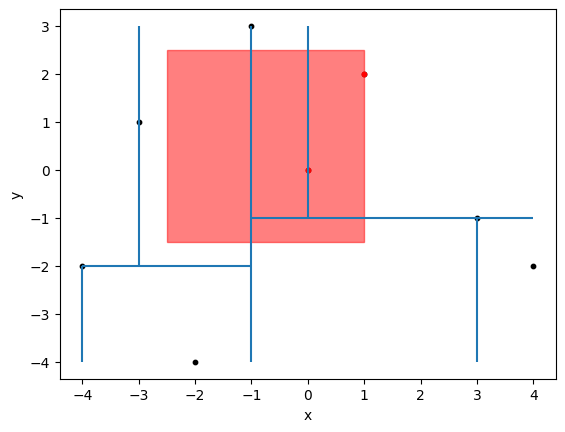
\includegraphics[width=\textwidth]{imgs/9}
        \column{0.5\textwidth}
        \begin{tikzpicture}[scale=0.8,level distance=1.5cm,
            level 1/.style={sibling distance=5cm},
            level 2/.style={sibling distance=2.5cm},
            level 3/.style={sibling distance=1.2cm}]
            \tikzstyle{vertex}=[circle,fill=black!25,inner sep=0pt,scale=0.5,minimum size=1.6cm]
            \tikzstyle{leaf}=[scale=0.5]
            \node[vertex]{$x=-1$}
                child{node[vertex]{$y=-2$}
                    child{node[vertex]{$x=-4$}
                        child{node[leaf]{$(-4, -2)$}}
                        child{node[leaf]{$(-2, -4)$}}
                    }
                    child{node[vertex]{$x=-2$}
                        child{node[leaf]{$(-3, 1)$}}
                        child{node[leaf]{$(-1, 3)$}}
                    }
                }
                child{node[vertex]{$y=-1$}
                    child{node[vertex]{$x=3$}
                        child{node[leaf]{$(3, -1)$}}
                        child{node[leaf]{$(4, -2)$}}
                    }
                    child{node[vertex]{$x=0$}
                        child{node[leaf]{$(0, 0)$}}
                        child{node[leaf]{$(1, 2)$}}
                    }
                };
        \end{tikzpicture}
    \end{columns}
\end{frame}


\begin{frame}{kd-drzewo -- analiza złożoności}
    Budując drzewo, trzeba w każdym kroku liczyć medianę, co odbywa się w czasie $\sO(n)$.
    Drzewo jest zrównoważone, więc z każdym podziałem zbiór zmniejsza się dwukrotnie,
    więc ostateczna złożoność wynosi $\sO(n \log n)$.

    \pause
    \begin{lemma}[o kd-drzewie]
        Dla zrównoważonego kd-drzewa o zamiennym podziale (czyli takim, gdzie punkt dzielący jest wybierany według różnych wymiarów dla różnych poziomów drzewa), dowolna pionowa lub pozioma prosta przecina $\sO(\sqrt n)$ komórek.
    \end{lemma}

    Złożoność
    \begin{enumerate}
        \item konstrukcji drzewa: $\sO(n\log n)$,
        \item zapytania: $\sO(\sqrt n + k)$,
        \item pamięciowa: $\sO(n)$.
    \end{enumerate}
\end{frame}

\section{Porównanie}

\begin{frame}{Porównanie}
    \centering
    \only<1,3,5>{
        \begin{tabular}{lll}
            \toprule
            & quadtree & kd-tree \\
            \midrule
            konstrukcja & $\sO(n\log\beta) $ & $\sO(n\log n)$ \\
            zapytania & $\sO(k\log\beta)$ & $\sO(\sqrt{n} + k)$ \\
            pamięć & $\sO(n\log\beta)$ & $\sO(n)$ \\
            \bottomrule
        \end{tabular}
    }
    \includegraphics<2>[width=0.65\textwidth]{../documentation/imgs/uniform_construction_time}
    \includegraphics<4>[width=0.65\textwidth]{../documentation/imgs/uniform_find_small_time}
    \includegraphics<6>[width=0.65\textwidth]{../documentation/imgs/pairs_construction_time}
\end{frame}

\end{document}